\documentclass[abstract=on,10pt,a4paper,bibliography=totocnumbered]{article}
\usepackage[paper=a4paper,left=35mm,right=35mm,top=25mm,bottom=30mm]{geometry}
\usepackage[doublespacing]{setspace}
\usepackage[english]{babel}
\usepackage[utf8]{inputenc}
\usepackage[round]{natbib}
\usepackage{amsmath}
\usepackage{colortbl}
\usepackage{amsfonts}
\usepackage{amssymb}
\usepackage{gensymb}
\usepackage{graphicx}
\usepackage{tikz}
\usepackage{enumerate}
\usepackage{enumitem}
\usepackage{subcaption}
\usepackage{booktabs}
\usepackage[hidelinks]{hyperref}
\usepackage[nameinlink]{cleveref}
% \usepackage{lineno}
\usepackage{multirow}
\usepackage{arydshln}
\usepackage[flushleft]{threeparttable}
\usepackage[nomarkers, nolists]{endfloat}
\usepackage[colorinlistoftodos]{todonotes}

%------------------------------------------------------------------------------
%	Some Styling
%------------------------------------------------------------------------------
% Creating some TikZ styles
\tikzset{
  nonterminal/.style = {rectangle
    , minimum size = 6mm
    , very thick
    , draw = black!
  }
}

% Changing the style of captions in figures etc.
\captionsetup{labelfont=bf, format=plain, font=small}

% Change how equations are referenced
\renewcommand{\theequation}{Equation \arabic{equation}}%

%------------------------------------------------------------------------------
%	Titlepage: Header
%------------------------------------------------------------------------------
\title{A Thee-Step Approach for Assessing Landscape Connectivity via Simulated
Dispersal: African Wild Dog Case Study}

% List of Authors
\author{
  David D. Hofmann\textsuperscript{1,2,\S} \and
  Gabriele Cozzi\textsuperscript{1,2} \and
  John W. McNutt\textsuperscript{2} \and
  Arpat Ozgul\textsuperscript{1} \and
  Dominik M. Behr\textsuperscript{1,2}
}

% Reduce spacing between authors
\makeatletter
\def\and{%
  \end{tabular}%
  \hskip -0.5em \@plus.17fil\relax
  \begin{tabular}[t]{c}}
\makeatother

% Current Date
% \date{\today}

% And here the masterpiece begins
\begin{document}

% Change page numbering
\pagenumbering{gobble}

% Required to be able to cite
\bibliographystyle{apalike}

% Create Titlepage
\maketitle

%------------------------------------------------------------------------------
%	Titlepage: Additional Info
%------------------------------------------------------------------------------
\begin{flushleft}

\vspace{0.5cm}

\textsuperscript{1} Department of Evolutionary Biology and Environmental
Studies, University of Zurich, Winterthurerstarsse 190, 8057 Zurich,
Switzerland.

\textsuperscript{2} Botswana Predator Conservation Program, Private Bag 13,
Maun, Botswana.

\textsuperscript{\S} Corresponding author (david.hofmann2@uzh.ch)

\vspace{4cm}

\textbf{Running Title:} Simulating Wild Dog Dispersal Trajectories to Assess
Landscape Connectivity

\vspace{0.5cm}

\textbf{Keywords:} dispersal, simulation, movement, integrated step selection
function, Kavango-Zambezi Transfrontier Conservation Area, landscape
connectivity, Lycaon pictus

\end{flushleft}

%------------------------------------------------------------------------------
%	Abstract
%------------------------------------------------------------------------------
% \newpage
% \begin{abstract}
% %------------------------------------------------------------------------------
% % Short Version
% %------------------------------------------------------------------------------
% \textbf{Short Version }
% The ability to disperse is contingent on a sufficient degree of landscape
% connectivity, which is why the identification and preservation of movement
% corridors that promote connectivity has become a task of extraordinary
% importance. Currently, ecologists rely on least-cost analysis or circuit theory
% to investigate connectivity, although both methods make several assumptions that
% are hardly met in reality. To address these issues, simulations from
% individual-based movement models have been proposed, yet a unified framework to
% simulate dispersal and quantify connectivity is lacking.
%
% Here, we propose a simple three-step approach that combines several
% already-existing methods to assess connectivity using simulated dispersal
% trajectories. In step one, we use integrated step selection functions to
% parametrize a mechanistic movement model rendering dispersal behavior. In step
% two, we apply the parametrized model as an individual-based movement model to
% simulate dispersal trajectories. In step three, we combine simulated
% trajectories into three complementary connectivity maps, each focusing on a
% different aspect of landscape connectivity.
%
% We showcase the application of the proposed approach using empirical data of
% dispersing African wild dogs (\textit{Lycaon pictus}) and assess landscape
% connectivity within the world's largest transboundary conservation area in
% Southern Africa. We thereby shed light into dispersing wild dogs' habitat and
% movement preferences, while also uncovering crucial dispersal corridors. With
% this analysis, we demonstrate that simulations from integrated step selection
% functions offer a simple, yet powerful alternative to traditional connectivity
% modeling techniques.
% \end{abstract}

\newpage
\begin{abstract}
%------------------------------------------------------------------------------
%  LONG VERSION
%------------------------------------------------------------------------------
Dispersal of individuals contributes to long-term population persistence, yet
requires a sufficient degree of landscape connectivity. To date, connectivity
has mainly been investigated using least-cost analysis and circuit theory, two
methods that make assumptions that are hardly applicable to dispersal.
Least-cost analysis assumes that animals move towards a known endpoint and are
knowledgeable about the most favorable route. Circuit theory presumes a complete
random walk and fails to incorporate directional persistence. While these
assumptions can be relaxed by simulating dispersal movements explicitly across
the landscape of interest, a unified approach for such simulations is lacking.

Here, we present a simple three-step approach to simulate dispersal movements
and to assess connectivity using empirical GPS movement data and environmental
habitat layers. In step one, we use integrated step selection functions to fit a
mechanistic movement model describing habitat and movement preferences of
dispersing individuals. In step two, we apply the parameterized movement model
to simulate dispersal trajectories. In step three, we derive three complementary
connectivity maps: a heatmap that highlights frequently traversed areas, a
betweenness map that pinpoints dispersal corridors, and a map of inter-patch
connectivity that indicates the presence and intensity of functional links
between habitat patches. As a case study, we applied the approach to GPS data
from dispersing individuals of the endangered African wild dog (\textit{Lycaon
pictus}) inhabiting the Kavango-Zambezi Transfrontier Conservation Area
(KAZA-TFCA).

Results from the case study show that wild dogs preferably disperse with
directional persistence in the vicinity to water bodies, through areas with
little human influence and sparse woodland cover. Dispersal simulations and
subsequent connectivity maps revealed several dispersal hotspots and corridors
across the extent of the KAZA-TFCA. Connectivity between NPs inside the
KAZA-TFCA was good, yet few dispersers successfully moved from Zambia's NPs into
neighboring areas. By rendering interactions between movement preferences and
habitat preferences, our movement model substantially outperformed a model that
omitted such interactions.

Ultimately, we show that a simulation-based approach that leverages on
step-selection functions offers a simple yet powerful alternative to traditional
connectivity modeling techniques. Such an approach not only makes fewer
biologically unrealistic assumptions but also permits a more mechanistic
understanding of dispersal and landscape connectivity. Our approach is thus
useful for a variety of applications in ecological, evolutionary, and
conservation research.

\end{abstract}

%------------------------------------------------------------------------------
%	Main Text
%------------------------------------------------------------------------------
\newpage

\onehalfspacing
\tableofcontents
\doublespacing

% Change page numbering
\newpage
\pagenumbering{arabic}

% Create linenumbers
% \linenumbers

\section{Introduction}

% Importance of Dispersal & Connectivity
\subsection{Importance of Connectivity \& Connectivity Models}
Dispersal of individuals is a vital process that allows species to maintain
genetic diversity \citep{Perrin.1999, Perrin.2000, Frankham.2002, Leigh.2012,
Baguette.2013}, rescue non-viable populations \citep{Brown.1977}, and colonize
unoccupied habitats \citep{Hanski.1999b, MacArthur.2001}. Importantly, the
ability to disperse depends on a sufficient degree of landscape connectivity
\citep{Fahrig.2003, Clobert.2012}, making the identification and protection of
dispersal corridors that promote connectivity a task of fundamental importance
\citep{Nathan.2008, Doerr.2011, Rudnick.2012}. Identifying dispersal corridors
not only necessitates a comprehensive understanding of the factors that limit
dispersal movements, but also an appropriate model to estimate connectivity
\citep{Baguette.2013, Vasudev.2015, Hofmann.2021}. To date, the most commonly
used models to assess connectivity are least-cost path analysis (LCPA;
\citealp{Adriaensen.2003}) and circuit theory (CT; \citealp{McRae.2006,
McRae.2008}). Unfortunately, both models rest on assumptions that appear
unsuitable for dispersers, calling for the development of alternative
approaches. One promising alternative is to assess landscape connectivity via
simulated dispersal trajectories generated from individual-based movement models
(IBMMs, \citep{Diniz.2019}).

% Issues with Both Methods
\subsection{Issues with Traditional Connectivity Models}
Traditional connectivity models make assumptions that are rarely met for
dispersers. LCPA, for instance, assumes that individuals move towards a
preconceived endpoint and choose a cost-minimizing route accordingly
\citep{Sawyer.2011, Abrahms.2017}. While this assumption may be justifiable for
migrating animals, it is unlikely to hold for dispersers, as dispersers
typically move across unfamiliar territory towards an unknown endpoint
\citep{Koen.2014, Cozzi.2020}. CT, on the contrary, posits that animals move
according to a random walk, entailing that autocorrelation between subsequent
movements cannot be rendered \citep{Diniz.2019}. For dispersers, however,
autocorrelated movements are regularly observed \citep{Cozzi.2020,
Hofmann.2021}, implying that dispersal trajectories are usually strongly
directional. Moreover, because both models require static permeability or
resistance surfaces as input, they are unable to reflect the temporal dimension
of dispersal, meaning that statements about the expected duration for moving
between habitat patches are impossible \citep{Martensen.2017, Diniz.2019}.

% What about IBMMs?
\subsection{What about IBMMs?}
The shortcomings inherent to LCPA and CT can be overcome by simulating dispersal
using IBMMs and by converting simulated trajectories into meaningful measures of
connectivity \citep{Diniz.2019}. In contrast to LCPA and CT, IBMMs allow to
explicitly simulate how individuals move across and interact with the
encountered landscape \citep{Kanagaraj.2013, Clark.2015, Allen.2016,
Hauenstein.2019, Zeller.2020}, as well as to render potential interactions
between movement behavior and habitat conditions \citep{Avgar.2016}. This
strictly shifts the focus from a structural to a more functional view on
connectivity \citep{Tischendorf.2000, Kanagaraj.2013, Hauenstein.2019}.
Furthermore, IBMMs generate movement sequentially, i.e. they generate a series
of steps, so that the temporal dimension of dispersal movements becomes explicit
and allows modeling autocorrelation between consecutive steps
\citep{Diniz.2019}. Finally, simulations from IBMMs do not enforce movement or
connections towards preconceived endpoints, thereby preventing biases arising
from misplaced endpoints. Despite these advantages, a unifying framework to
simulate dispersal and assess connectivity using IBMMs is lacking. Considering
the large number of subjective decisions entailed by IBMMs, an approach that
streamlines and unifies the application of dispersal simulations to assess
connectivity will, however, be critical to safeguard interspecfic comparability
and reproducability.

% Proposed Solution: Three-Step approach
\subsection{Proposed Solution: Three-Step Approach}
Here, we propose and exemplify a simple three-step approach for simulating
dispersal and assessing landscape connectivity (\Cref{GraphicalAbstract}). In
step one, we combine GPS movement data of dispersing individuals with relevant
habitat covariates to fit a mechanistic movement model using integrated step
selection functions (ISSFs, \citealp{Avgar.2016}). ISSFs allow inference on the
study species' habitat kernel (i.e. habitat preferences), its movement kernel
(i.e. movement preferences/capabilities), and potential interactions between the
two \citep{Avgar.2016, Fieberg.2021}. In step two, we simulate individual
dispersal trajectories using the parametrized movement model. Comparable
simulations have already been applied to estimate steady-state utilization
distributions of resident individuals \citep{Potts.2013, Signer.2017} and to
model landscape connectivity, yet disregarding interdependencies between habitat
and movement kernels \citep{Clark.2015, Zeller.2020}. Finally, in step three, we
convert simulated trajectories into three complementary connectivity maps, each
highlighting a different aspect of connectivity; (i) a heatmap revealing areas
that are frequently traversed by dispersers (e.g. \citealp{Hauenstein.2019,
Zeller.2020}), (ii) a betweenness-map delineating dispersal corridors and
bottlenecks (e.g. \citealp{BastilleRousseau.2018}), (iii) and a map of
inter-patch connectivity, depicting the presence and intensity of specific
connections, as well as the average dispersal duration required for the
realization of those connections (e.g. \citealp{Gustafson.1996,
Kanagaraj.2013}).

% Introduction of the study species
\subsection{Case Study}
We showcase the application of the proposed approach (\Cref{GraphicalAbstract})
using GPS movement data collected on dispersing individuals of the endangered
African wild dog (\textit{Lycaon pictus}). The African wild dog is a highly
mobile species whose population persistence heavily relies on the availability
of large, natural or semi-natural landscapes and a sufficient degree of
connectivity among remaining subpopulations. Once common throughout sub-Saharan
Africa, this species has disappeared from much of its historic range, largely
due to human persecution, habitat fragmentation, and disease outbreaks
\citep{Woodroffe.2012}. Wild dogs typically disperse in single-sex coalitions
\citep{McNutt.1996, Behr.2020} and are capable of dispersing several hundred
kilometers \citep{DaviesMostert.2012, Masenga.2016, Cozzi.2020}. Although
previous studies have investigated connectivity using LCPA \citep{Hofmann.2021}
or CT \citep{Brennan.2020}, a more comprehensive and mechanistic understanding
of connectivity is missing for this species (but see \citealp{Creel.2020}). With
fewer than 6,000 free-ranging wild dogs remaining in fragmented subpopulations
\citep{Woodroffe.2012}, reliable information on landscape connectivity is
essential for the conservation of this endangered carnivore. Here, we use GPS
data of 16 dispersing wild dogs originating from a free-ranging population in
northern Botswana to parametrize a mechanistic movement model, which we then
employed to simulate 80,000 dispersal trajectories across the landscape of the
world's largest transboundary conservation area, the Kavango-Zambezi
Transfrontier Conservation Area (KAZA-TFCA). We anticipated that simulations
based on our three-step approach would overcome several of the above highlighted
conceptual shortcomings of traditional connectivity models and provide a more
comprehensive view on dispersal behavior and landscape connectivity.

\begin{figure}[htbp]
  \begin{center}
    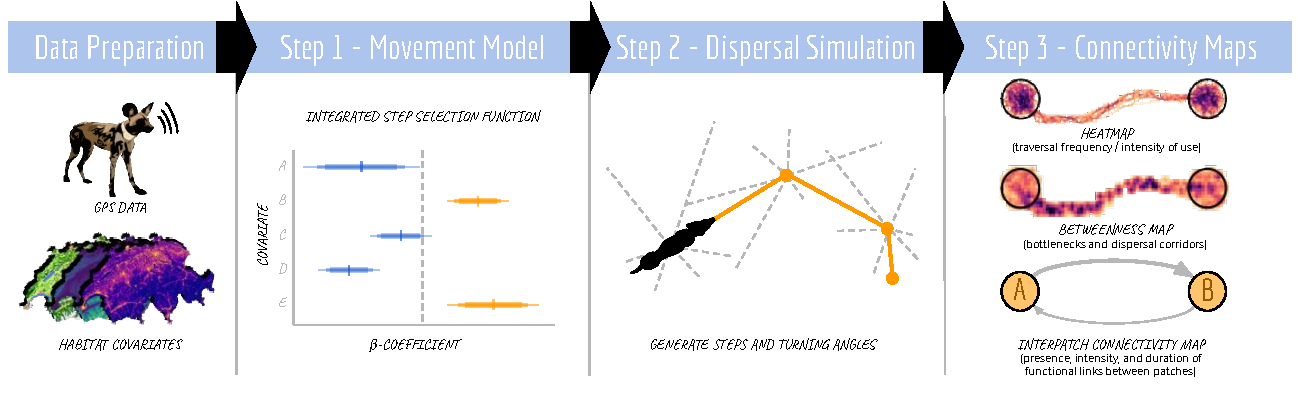
\includegraphics[width = \textwidth]{99_GraphicalAbstract2.pdf}
    \caption{Flowchart of the simulation-based connectivity analysis as proposed
    in this article. First, GPS data and habitat covariates must be
    collected. The combined data is then analyzed in an integrated step
    selection model, which enables the parametrization of the focal species'
    habitat and movement kernels and results in a mechanistic movement model.
    The parametrized model is then treated as an individual-based movement model
    and used to simulate dispersal trajectories. Ultimately, simulated
    trajectories serve to produce a set of maps that are pertinent to landscape
    connectivity. This includes a heatmap, indicating the traversal frequency
    across each spatial unit of the study area, a betweenness map, highlighting
    movement corridors and bottlenecks, and, finally, an inter-patch
    connectivity map, where the frequency of connections and their average
    duration can be depicted.}
    \label{GraphicalAbstract}
  \end{center}
\end{figure}

\section{Methods}
\subsection{Study Area}
Our simulation of dispersal trajectories and assessment of connectivity spanned
across the entire Kavango-Zambezi Transfrontier Conservation Area (KAZA-TFCA),
an area of approximately 1.3 Mio. km\textsuperscript{2} (\Cref{StudyArea}a and
b). The KAZA-TFCA is the world's largest transboundary conservation area and
comprises parts of Angola, Botswana, Namibia, Zimbabwe, and Zambia, thus hosting
a rich diversity of landscapes, ranging from savannah to grassland and from dry
to moist woodland habitats. In its center lies the Okavango Delta, a dominant
hydro-geographical feature and the world's largest flood-pulsing inland delta.
Large portions of the KAZA-TFCA are formally protected in the form of national
parks (NPs) or other protected areas, yet a considerable portion of the
landscape is still human-dominated (e.g. roads, agricultural sites, and
settlements).

\begin{figure}[h]
  \begin{center}
    \begin{tikzpicture}
        \node[anchor=south west,inner sep=0] (image) at (0,0,0) {
        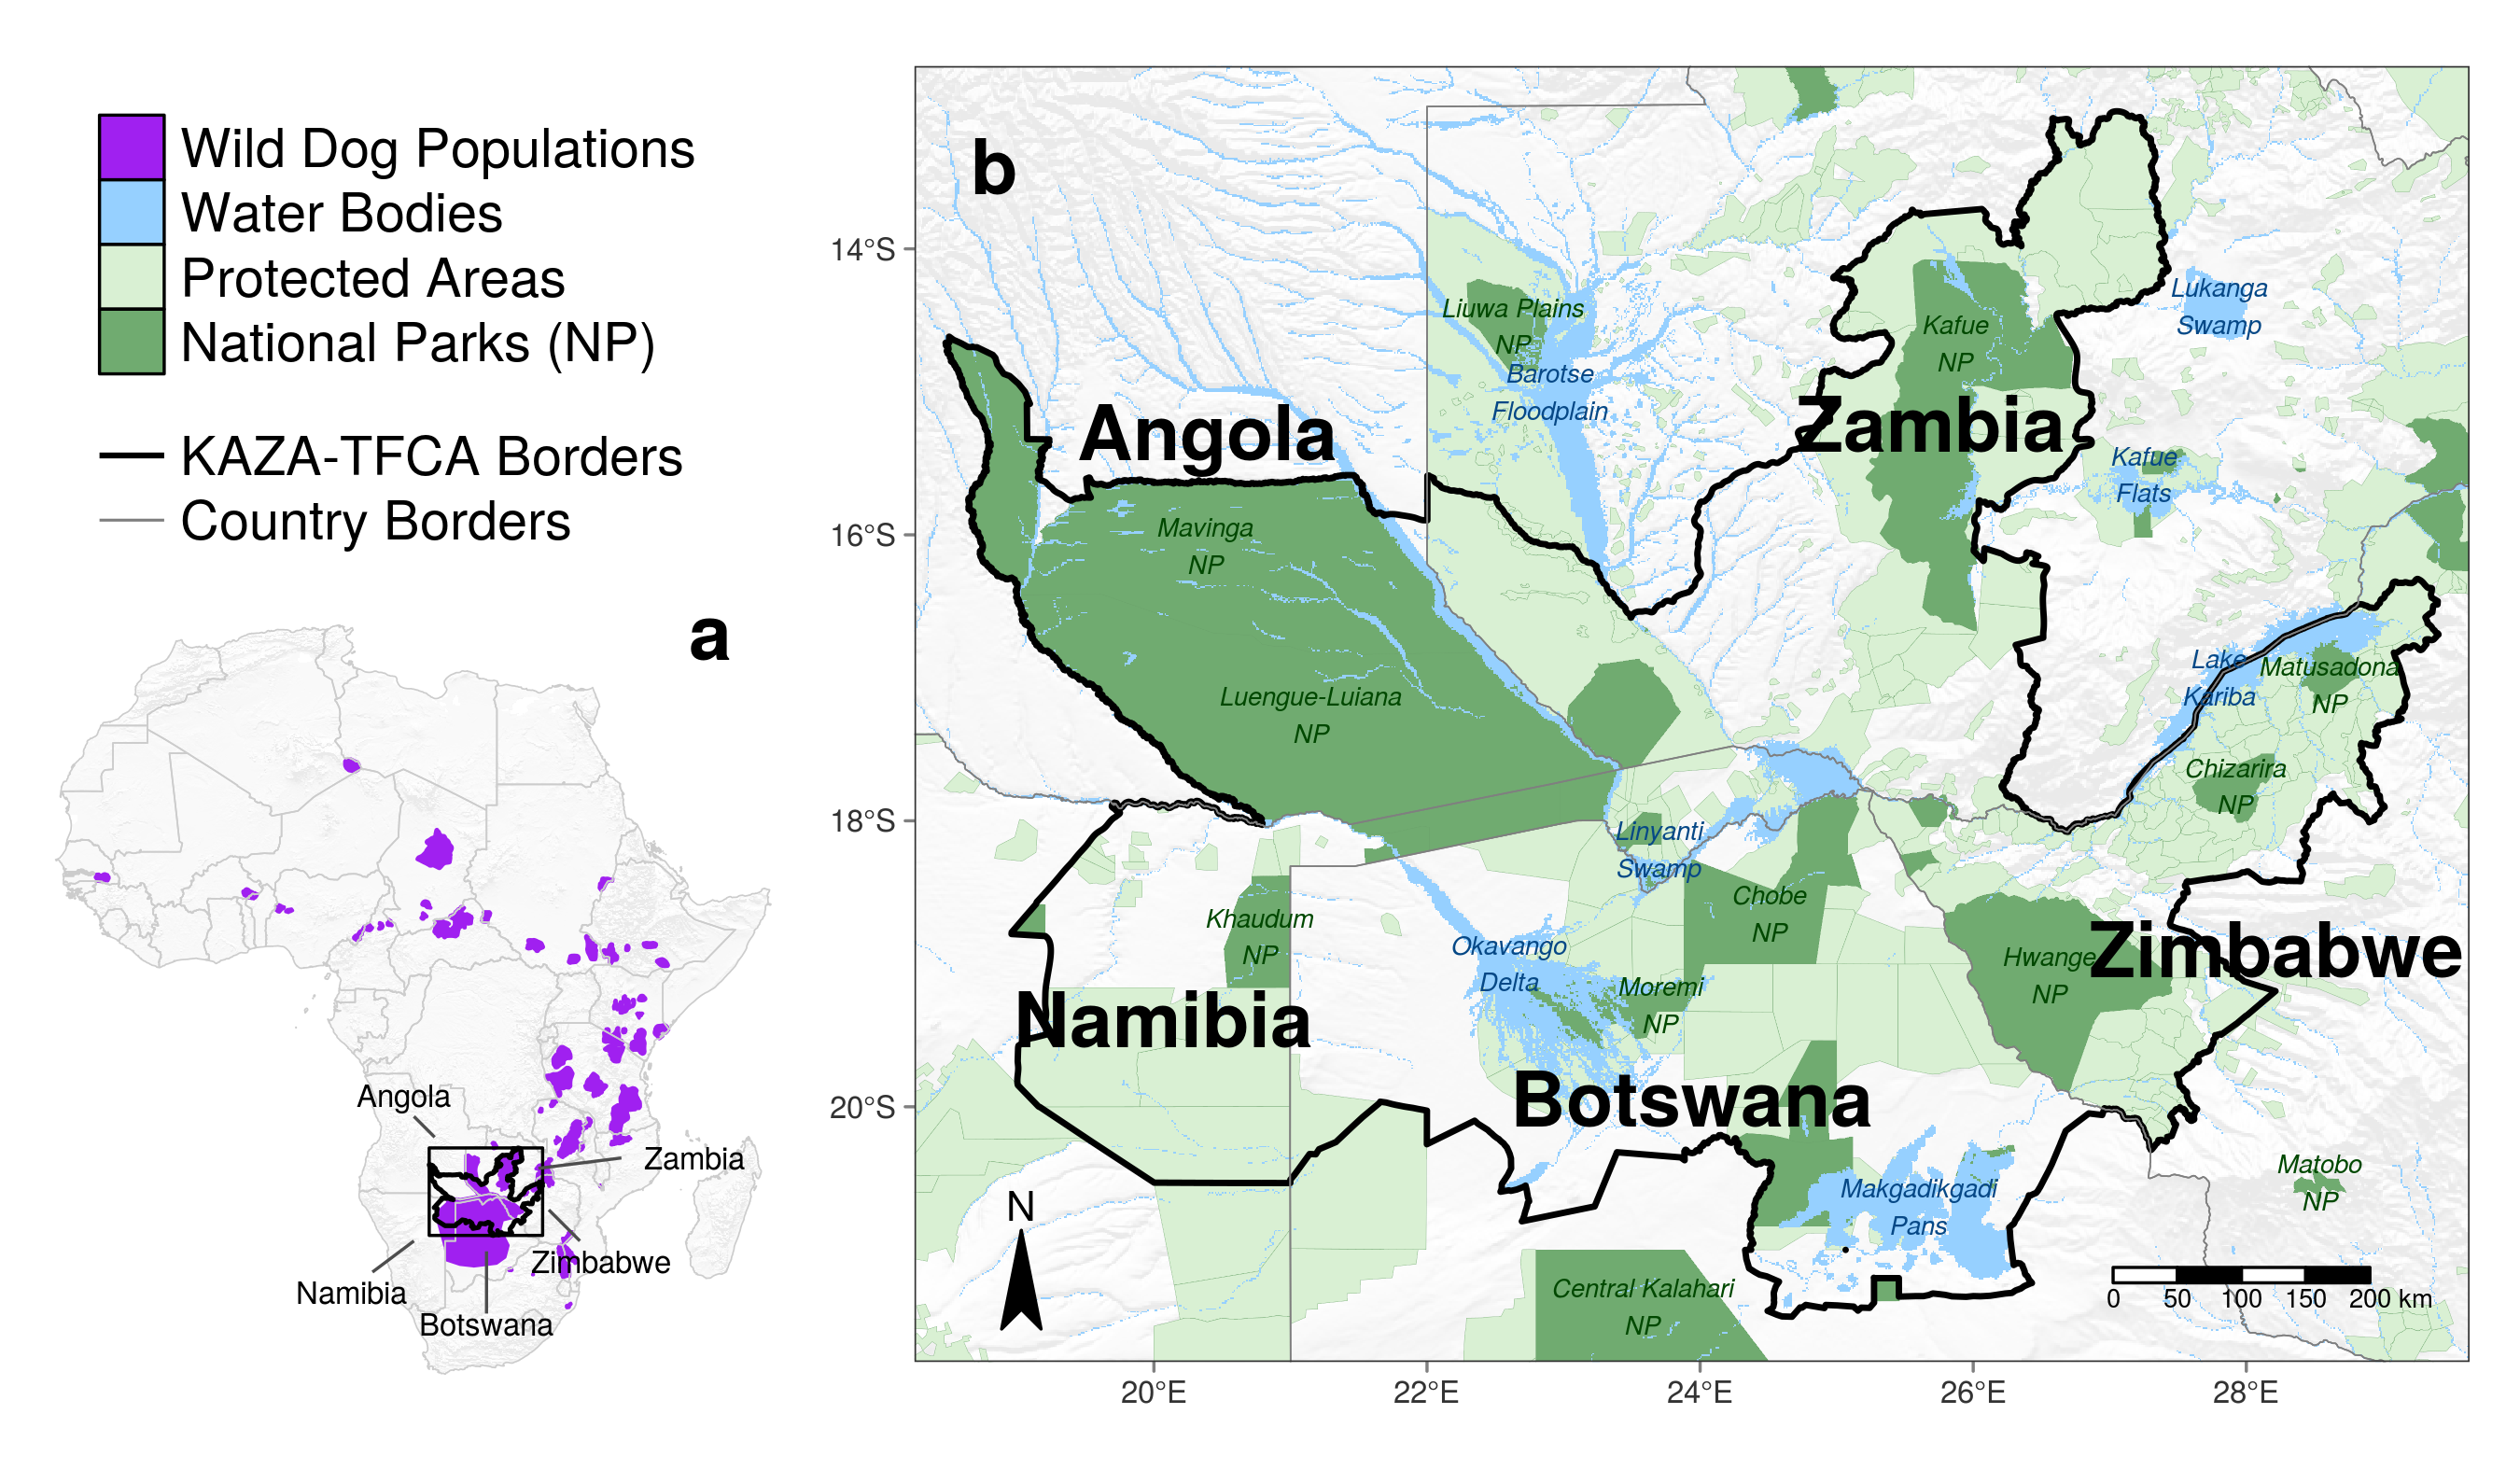
\includegraphics[width=\textwidth]{99_StudyArea.png}
        };
        \begin{scope}[x={(image.south east)},y={(image.north west)}]
            % % next four lines will help you to locate the point needed by forming a grid.
            % % comment these four lines in the final picture.
            % \draw[help lines,xstep=.1,ystep=.1] (0,0) grid (1,1);
            % \draw[help lines,xstep=.05,ystep=.05] (0,0) grid (1,1);
            % \foreach \x in {0,1,...,9} { \node [anchor=north] at (\x/10,0) {0.\x}; }
            % \foreach \y in {0,1,...,9} { \node [anchor=east] at (0,\y/10) {0.\y};}
            % % upto here
            \draw[densely dotted, blue] (0.169, 0.222) -- (0.364, 0.955);
            \draw[densely dotted, blue] (0.169, 0.157) -- (0.364, 0.074);
        \end{scope}
    \end{tikzpicture}
    \caption{Illustration of the study area located in southern Africa. (a) The
    study area was confined by a bounding box spanning the entire KAZA-TFCA
    which comprises parts of Angola, Namibia, Botswana, Zimbabwe, and Zambia.
    (b) The KAZA-TFCA currently represents the world's largest terrestrial
    transfrontier conservation area, covering a total area of 520'000
    km\textsuperscript{2}. Its main purpose is to re-establish connectivity
    between already-existing NPs (dark green) and other protected areas (light
    green).}
    \label{StudyArea}
  \end{center}
\end{figure}

\subsection{Data Collection and Preparation}
\subsubsection{GPS Data}
We collected GPS movement data on 16 dispersing coalitions of African wild dogs
(7 female and 9 male coalitions) between 2011 and 2019 from a free-ranging
population in northern Botswana (details on the data collection can be found in
\cite{Cozzi.2020} and \cite{Hofmann.2021}). To delineate periods of dispersal,
we determined the exact timing of emigration from the natal pack and settlement
in a new territory using direct field observations and through visual inspection
of the net squared displacement (NSD) metric. The NSD metric measures the
squared Euclidean distance of a GPS relocation to a reference point
\citep{Borger.2012}, which we set to the center of the territory of each
dispersers' natal pack. Thus, dispersal was deemed to have started once an
individual left its natal territory and ended once the NSD metric remained
constant, indicating settlement. Because behavior during dispersal is more
pertinent to landscape connectivity than behavior during residence
\citep{Elliot.2014, Abrahms.2017}, we only considered data collected during
dispersal for our analysis. During dispersal, GPS collars recorded a fix every 4
hours and regularly transmitted data over the Iridium satellite system. To
ensure regular time intervals between GPS fixes, we removed any fixes that were
not successfully obtained at the desired 4-hour schedule (allowing for a
tolerance of \( \pm \) 15 minutes). We then converted the fixes (n = 4'169) into
steps, where each step represented the straight-line movement between two
consecutive GPS fixes \citep{Turchin.1998}.

\subsubsection{Habitat Covariates}
We represented the physical landscape in our study area by the habitat
covariates \textit{water-cover, distance-to-water, woodland-cover,
shrub/grassland-cover, and human-influence}. To render the seasonal dynamics in
water-cover of major water bodies for the extent of the Okavango Delta, we
applied an algorithm that enabled us to obtain weekly updated raster-layers for
water-cover and distance-to-water from MODIS satellite imagery
\citep{Wolski.2017, Hofmann.2021}. This algorithm is now implemented in the
\textsf{floodmapr} package (available on GitHub;
\url{https://github.com/DavidDHofmann/floodmapr}). To ensure a consistent
resolution across habitat covariates, we coarsened or interpolated all layers to
a resolution of 250 m x 250 m. A detailed description of how we prepared each
habitat covariate is provided in \cite{Hofmann.2021}.

Besides habitat covariates, we computed movement metrics that we used as
movement covariates in the ISSF models \citep{Avgar.2016, Fieberg.2021}.
Specifically, we computed for each step the step length (\textsf{sl}), its
natural logarithm (\textsf{log(sl)}), and the cosine of the relative turning
angle (\textsf{cos(ta)}). Moreover, we created the binary variable
\textsf{LowActivity}, indicating whether a step was realized during periods of
low wild dog activity (09:00 to 17:00 local time) or high wild dog activity
(17:00 to 09:00 local time, following \citealp{Cozzi.2012}). We performed all
data preparations, spatial computations, and statistical analysis in R, version
3.6.6 \citep{R.2020}. Some helper functions were written in {\tt C++} and
imported into {\tt R} using the {\tt Rcpp} package \citep{Eddelbuettel.2011,
Eddelbuettel.2013}.

\subsection{Step 1 - Movement Model}
We used ISSFs \citep{Avgar.2016} to parametrize a mechanistic movement model for
dispersing wild dogs. More specifically, we paired each realized (i.e. observed)
step with 24 random steps, so that a realized step plus its 24 random steps
formed a 25-step-stratum that received a unique identifier. As suggested by
\cite{Avgar.2016}, we generated random steps by sampling random turning angles
from a uniform distribution (\(-\pi, +\pi\)) (which is equivalent to a von Mises
distribution with location and concentration parameters; \(\mu = \kappa = 0\))
and step lengths from a gamma distribution that was fitted to realized steps
(scale \(\theta\) = 6'308 and shape \(k\) = 0.37).

Along each realized and random step, we extracted values from the habitat
covariate layers using the {\tt velox} package \citep{Hunziker.2021} and we
computed averages of each covariate along the steps. We further calculated the
movement metrics \textsf{sl}, \textsf{log(sl)}, and \textsf{cos(ta)} for each
step. To facilitate model convergence, we standardized all continuous covariates
to a mean of zero and a standard deviation of one. Correlations among covariates
were low (\(|r| < 0.6\); \citealp{Latham.2011}), so we retained all of them for
modeling.

To contrast realized steps (scored 1) and random steps (scored 0), we assumed
that animals assigned a selection score \(w(x)\) to each step (\ref{EQ1};
\citealp{Fortin.2005}). \(w(x)\) depended on the step's associated covariates
(\(x_1, x_2, ..., x_n\)) and on the animal's preferences (i.e. relative
selection strengths; \citealp{Avgar.2017}) towards these covariates (\(\beta_1,
\beta_2, ..., \beta_n\)):

\begin{equation}
\label{EQ1}
  w(x) = exp(\beta_1 x_1 + \beta_2 x_2 + ... + \beta_n x_n)
\end{equation}

\noindent The probability of a step \(i\) being realized was then contingent on
the step's selection score, as well as on the selection scores of all other step
in the same stratum:

\begin{equation}
\label{EQ2}
  P(Y_{i} = 1 | Y_{1} + Y_{2} + ... + Y_{i} = 1) =
  \frac{w(x_{i})}{w(x_{1}) + w(x_{2}) + ... + w(x_{i})}
\end{equation}

\noindent To estimate preferences (i.e. the \(\beta\)-coefficients), we used
mixed effects conditional logistic regression analysis \citep{Muff.2020} that we
implemented using the r-package {\tt glmmTMB} \citep{Brooks.2017}. The method
introduced by \cite{Muff.2020} allows to model random slopes, yet requires to
fix the variance of the stratum specific intercept to a large value. Hence we
fixed the stratum specific intercept variance to an arbitrary high value of \(10
^ 6\). We used disperser identity to model random slopes for all covariates.

The covariate structure of the movement model was based on a habitat selection
model that was previously developed for dispersing wild dogs (hereafter referred
to as \textit{based model}, \citealp{Hofmann.2021}). In the base model, no
interactions among habitat covariates and movement covariates were considered.
Hence, we expanded the base model and allowed for interactions between all
movement covariates and habitat covariates, thus reflecting that movement
behavior may depend on habitat conditions (details in Appendix A1). To determine
the most parsimonious movement model among model candidates, we ran stepwise
forward model selection based on Akaike's Information Criterion (AIC,
\citealp{Burnham.2002}). Finally, we validated the predictive power of the most
parsimonious model using k-fold cross-validation for case-control studies as
described in \cite{Fortin.2009}. This validation proves a significant prediction
in case the Spearman rank correlation of predicted step-ranks and associated
frequencies under the movement model is significantly greater than under the
assumption of random preferences (details in Appendix A2).

\subsection{Step 2 - Dispersal Simulation}
We used the most parsimonious movement model to simulate individual dispersal
trajectories within the study area. The simulation of a dispersal trajectory
resembled an ``inverted'' ISSF and was set up as follows. (1) We defined a
random source point and assumed a random initial orientation of the simulated
animal. (2) Starting from the source point, we generated 25 random steps by
sampling turning angles from a uniform distribution (\(-\pi, +\pi\)) and step
lengths from our fitted gamma distribution. Similarly to the empirical data,
each random step represented a 4 hours straight-line movement. To prevent
unreasonably large steps, we restricted sampled step lengths to a maximum of 35
km (i.e. the farthest dispersal distance traveled within 4 hours in our data).
(3) Along each random step, we extracted and averaged values from the different
habitat covariate layers and calculated movement covariates (as explained under
Step 1). To ensure compatible scales with the fitted movement model, we
standardized extracted values using means and standard deviations from the
empirical data. (4) We applied the parametrized movement model to predict the
selection score \(w(x)\) for each step using \ref{EQ1} and we converted
predicted scores into probabilities using \ref{EQ2}. (5) We randomly sampled one
of the generated random steps based on assigned probabilities and determined the
animal's new position. We repeated steps (2) to (5) until 2,000 steps were
realized.

To mitigate edge effects and to deal with random steps leaving the study area,
we followed \cite{Koen.2010} and artificially expanded all covariate layers by a
100 km wide buffer zone. Within the buffer zone, we randomized covariate values
by resampling values from the original covariate layers. Through this buffer
zone, simulated dispersers were able to leave and re-enter the main study area.
In cases where random steps crossed the outer border of this buffer zone, we
resampled steps until they fully lied within the buffer zone, essentially
forcing individuals to remain within the expanded study area.

For the simulation, we distributed 80,000 source points within the study area.
Of these, 50,000 were located inside protected areas that were larger than the
average home range of resident wild dog packs (i.e. \(>\) 700
km\textsuperscript{2}; \citealp{Pomilia.2015}), while the remaining 30,000 were
placed randomly inside the buffer zone, mimicking potential immigration into the
study area (Figure S1).

To ensure reliable connectivity estimates, we determined the number of simulated
dispersal trajectories required for connectivity to reach a ``steady state''
across the entire study area. For this purpose, we distributed 1,000 rectangular
``checkpoints'', each with an arbitrary extent of 5 km x 5 km at random
coordinates within the study area (excluding the buffer). We then determined the
relative frequency at which each checkpoint was traversed by simulated dispersal
trajectories (hereafter referred to as relative traversal frequency) as we
gradually increased the number of simulated trajectories from 1 to 50,000. To
assess variability in the relative traversal frequency, we repeatedly subsampled
100 times from all 50'000 trajectories and computed the mean traversal frequency
across replicates, as well as its 95\% prediction-interval for each checkpoint.
We considered connectivity to have reached a steady state once the width of the
prediction-interval dropped below a value of 0.01 for all checkpoints.

\subsection{Step 3 - Connectivity Maps}
\subsubsection{Heatmap}
To identify dispersal hotspots within the study area, we created a heatmap
indicating the absolute frequency at which each raster-cell was traversed by
simulated dispersal trajectories (e.g. \citealp{Peer.2008, Hauenstein.2019,
Zeller.2020}). Specifically, we rasterized all simulated trajectories onto a
raster with 1 km x 1 km resolution and tallied resulting layers into a single
map. If the same trajectory crossed a raster-cell twice, we only counted it once
to reduce biases due to individuals that were surrounded by unfavorable habitat
and therefore ``moved in circles''. To achieve high performance rasterization,
we used the R-package {\tt terra} \citep{Hijmans.2021b}.

\subsubsection{Betweenness Map}
To pinpoint movement corridors and bottlenecks, we converted simulated
trajectories into a network and calculated betweenness scores for all
raster-cells in the study area \citep{BastilleRousseau.2018}. Betweenness is a
pertinent metric for connectivity as it measures how often a specific
network-node (in our case a raster-cell) lies on a shortest path between any
other pair of nodes \citep{BastilleRousseau.2018}. To convert simulated
trajectories into a network, we followed \cite{BastilleRousseau.2018} and
overlaid the study area (including the buffer) with a 5 km x 5 km raster, where
the center of each raster-cell served as node in the final network. To identify
edges (i.e. connections) between the nodes, we used the simulated trajectories
and determined all transitions occurring from one node to another, as well as
the frequency at which those transitions occurred. This resulted in an edge-list
that we translated into a weighted network using the r-package {\tt igraph}
\citep{Gabor.2006}. The weight of each edge was determined by the frequency of
transitions, yet because {\tt igraph} handles edge weights (\(\omega\)) as
costs, we inverted the traversal-frequency through each raster-cell by applying
\(\omega = \frac{mean(Traversal Frequency)}{Traversal Frequency_i}\).
Consequently, regularly used edges received small weights (i.e. low costs) and
vice versa. Finally, we used the weighted network to calculate betweenness
scores for all network nodes.

\subsubsection{Inter-Patch Connectivity Map}
To examine the presence and intensity of functional links (i.e. connections)
between specific patches inside the KAZA-TFCA, we calculated inter-patch
connectivity between NPs (e.g. \citep{Gustafson.1996, Kanagaraj.2013}). The
decision to only consider NPs as potential ``patches'' was purely out of
simplicity and does not imply that connections between other protected areas do
not occur. To quantify inter-patch connectivity, we computed the relative
frequency at which dispersers originating from one NP successfully moved into
another NP. We considered movements as successful if an individual's dispersal
trajectory intersected with the target NP at least once. For each trajectory we
also recorded the number of steps required to reach the first intersection with
the respective NP, allowing us to compute the average dispersal durations from
one NP to another. In summary, we determined \textit{if} and \textit{how often}
dispersers moved between certain NPs, as well as \textit{how long} individuals
had to move to make these connections.

\section{Results}
\subsection{Movement Model}
The most parsimonious movement model consisted of movement covariates, habitat
covariates and several of their interactions, suggesting that movement behavior
during dispersal depended on habitat conditions (\Cref{MovementModel}a, Table S1
and Table S2). Although multiple models received an AIC weight > 0 (Table S1),
we only considered results from the most parsimonious model for simplicity. This
decision only marginally influenced subsequent steps as all models with positive
AIC weights retained similar covariates (Table S1). Plots that aid with model
interpretation are provided in Figure S2. Under average conditions, dispersing
wild dogs avoided moving through water, woodlands, and areas dominated by
humans, but preferred shrublands or grasslands (\Cref{MovementModel}a).
Dispersers realized shorter steps (indicating slower movements) in areas covered
by water or woodland, while realizing larger steps in areas dominated by shrubs
or grass (\Cref{MovementModel}a). Moreover, dispersing wild dogs moved faster
during twilight and at night (i.e. between 17:00 and 09:00 o'clock) than during
the rest of the day (\Cref{MovementModel}a). Although dispersers showed a
preference for directional movements (i.e. low turning angles), especially when
moving quickly, they did less so in proximity to humans or water, resulting in
more tortuous movements in such areas (\Cref{MovementModel}a).

The k-fold cross-validation of the movement model showed that the final model
substantially outperformed a random guess and suggested reliable predictions
(i.e. confidence intervals of \(\bar{r}_{s, realized}\) and \(\bar{r}_{s,
random}\) did not overlap). Moreover, the model correctly assigned high
selection scores to realized steps (\Cref{MovementModel}b), indicating a good
fit between predictions and observations. Compared to the base model
(\(\bar{r}_{s, realized} = -0.55; 95\%-CI = [-0.57, -0.52]\);
\citealp{Hofmann.2021}), the inclusion of several interactions between movement
and habitat covariates significantly improved model performance (\(\bar{r}_{s,
realized} = -0.65; 95\%-CI = [-0.67, -0.64]\).

\begin{figure}
  \begin{center}
    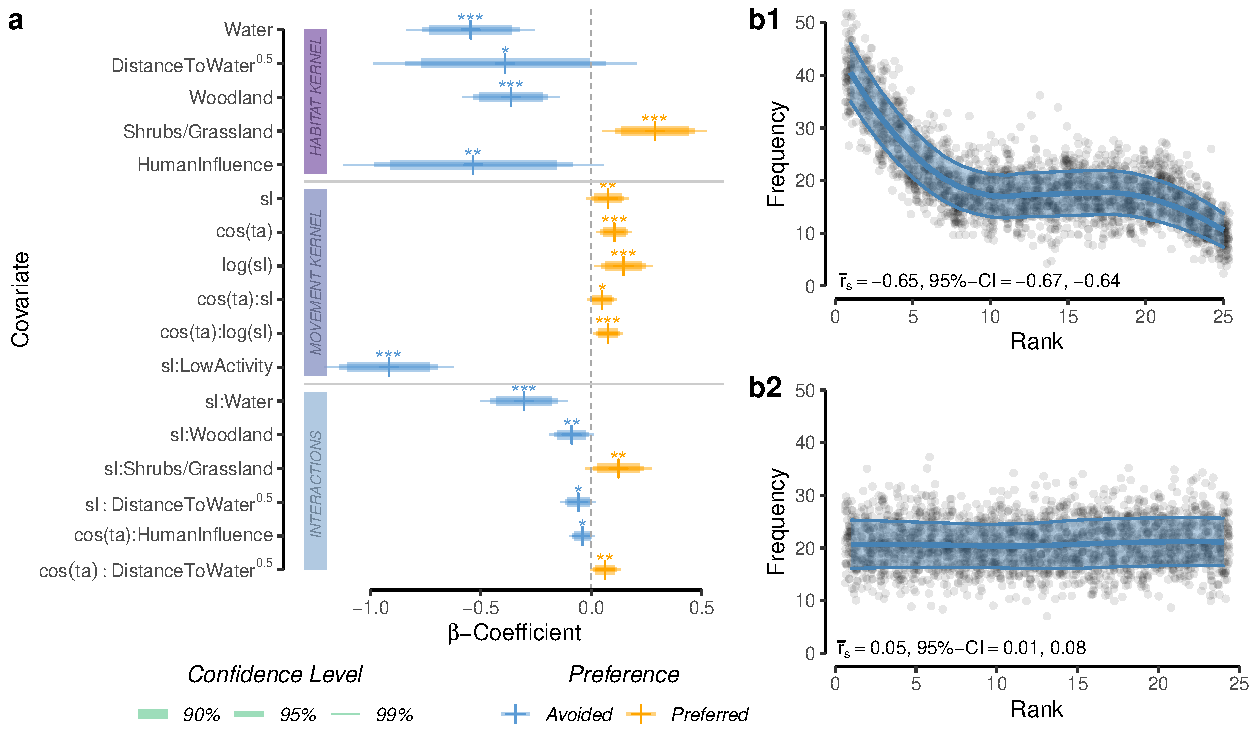
\includegraphics[width=\textwidth]{99_MovementModel}
    \caption{(a) Most parsimonious movement model for dispersing wild dogs. The
    model comprises a habitat kernel, a movement kernel, as well as their
    interactions. The horizontal line segments delineate the 90\%, 95\%, and
    99\% confidence-intervals for the respective \(\beta\)-coefficients.
    Significance codes: * \(p < 0.10\), ** \(p < 0.05\), *** \(p < 0.01\). (b)
    Results from the k-fold cross validation procedure. The upper plot shows
    rank frequencies of realized steps according to model predictions with known
    preferences, whereas the lower plot shows rank frequencies of realized steps
    when assuming random preferences. The blue ribbon shows the prediction
    interval around a loess smoothing regression that we fitted to ease the
    interpretation of the plots. The significant correlation between rank and
    associated frequency in (b1) highlights that the most parsimonious model
    successfully outperforms a random guess (b2) and assigns comparably high
    selection scores to realized steps.}
    \label{MovementModel}
  \end{center}
\end{figure}

\subsection{Dispersal Simulation}
Dispersal simulations based on the most parsimonious movement model proved
useful for assessing landscape connectivity. Of the 50,000 simulated dispersal
trajectories with starting point within the main study area, only 4.5\% reached
a map boundary, suggesting minimal biases due to boundary effects. Moreover, our
examination of the relative traversal frequency across all checkpoints showed
that connectivity reached a steady state after 10,500 simulated dispersal
trajectories (Figure S3). Although variability in relative traversal frequency
kept decreasing as we increased the number of simulated dispersers, the marginal
benefit of additional trajectories diminished quickly (Figure S3).

\subsection{Heatmap}
The heatmap (\Cref{Heatmap}), which resulted from the sum of all simulated
dispersal trajectories, showed that several extensive regions within the
KAZA-TFCA were frequently traversed by dispersing wild dogs (median traversal
frequency inside KAZA-TFCA = 166, IQR = 274, Figure S6a), whereas areas beyond
the KAZA-TFCA boundary were rarely visited (median traversal frequency outside
KAZA-TFCA = 61, IQR = 133, Figure S6a). Most notably, the region in northern
Botswana south of the Linyanti swamp appeared as highly frequented dispersal
hotspot (median traversal frequency = 987, IQR = 558). Nevertheless, the
presence of extensive water bodies, such as the Okavango Delta, the Makgadikgadi
Pan, and the Linyanti swamp, restricted dispersal movements and limited realized
connectivity within the KAZA-TFCA. Similarly, high human density, roads, and
agricultural activities in Zambia's and Zimbabwe's part of the KAZA-TFCA limited
dispersal movements in those countries. Outside the KAZA-TFCA, the most heavily
used regions included the areas inside the Central Kalahari NP in Botswana, the
area south-west of the Khaudum NP in Namibia, and the area surrounding the Liuwa
Plains NP in Zambia. Although the heatmap facilitated the identification of
areas frequently traversed by simulated dispersers, it seemed impractical to
pinpoint dispersal corridors.

\begin{figure}
  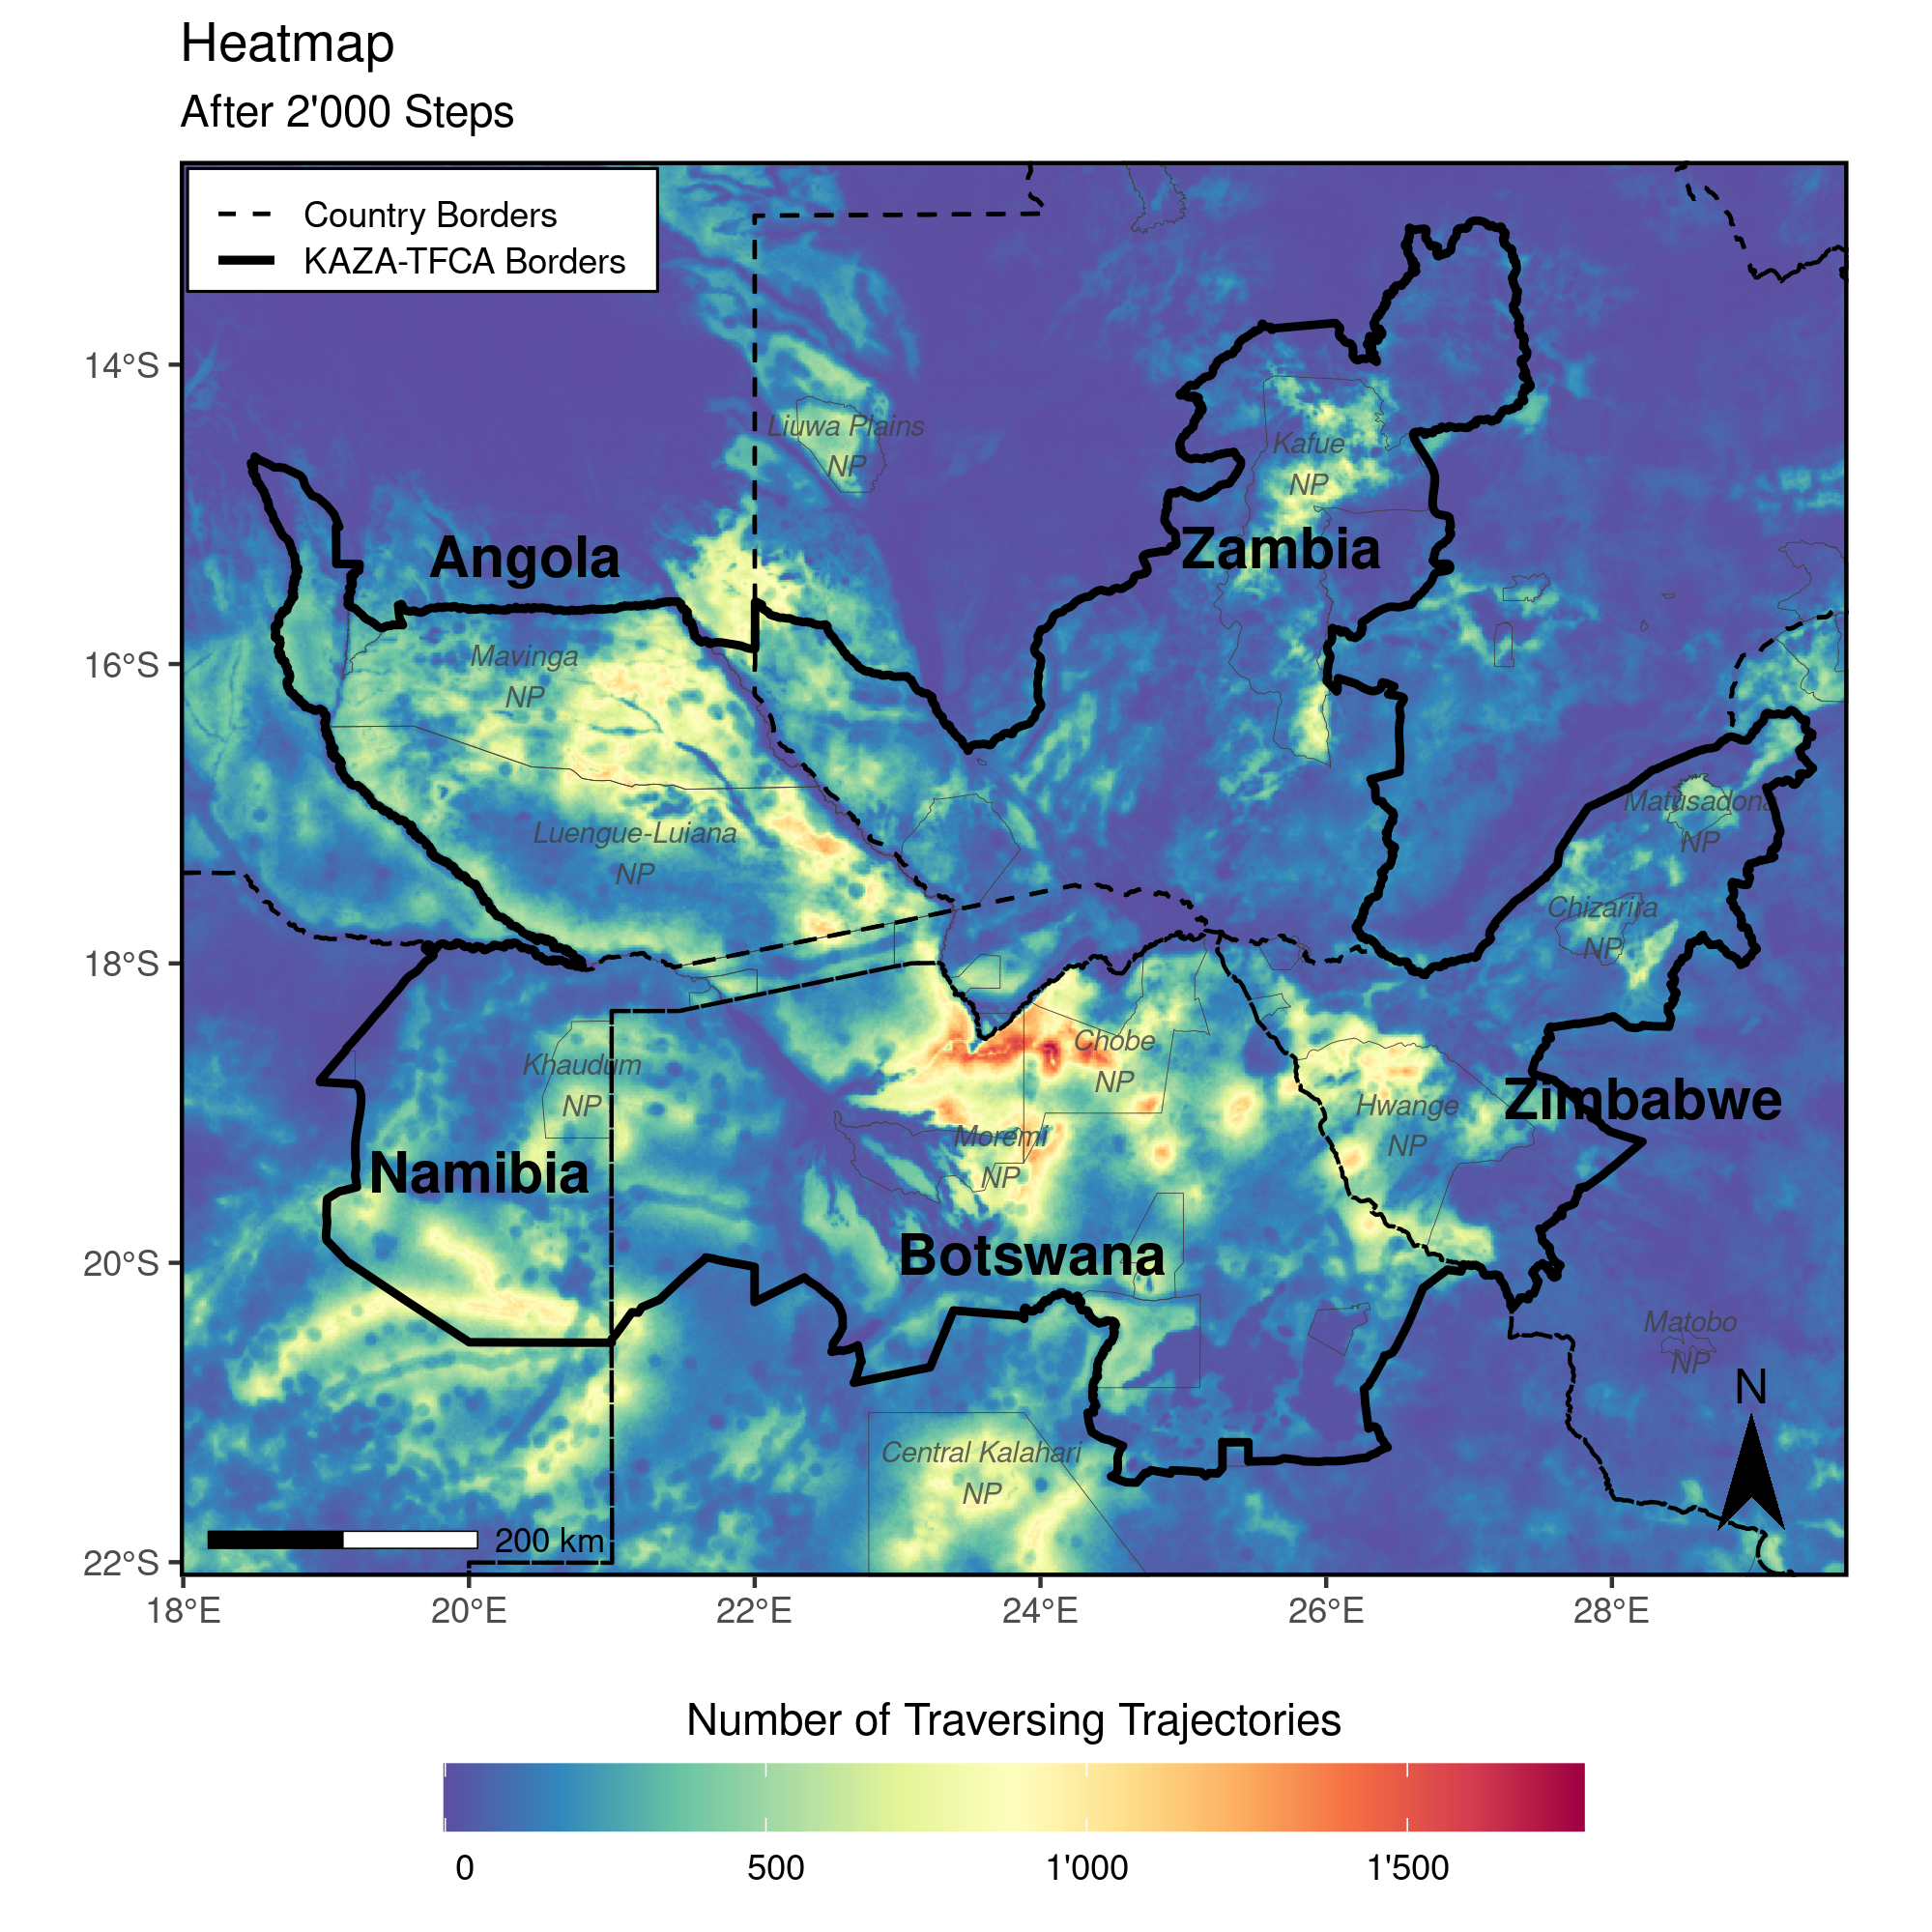
\includegraphics[width=\textwidth]{99_Heatmap.png}
  \caption{Heatmap showing traversal frequencies of 80'000 simulated dispersers
  moving 2'000 steps across the KAZA-TFCA. Simulations were based on an
  integrated step selection model that we fitted to the movement data of
  dispersing African wild dogs. To generate the heatmap, we rasterized and
  tallied all simulated trajectories. Consequently, the map highlights areas
  that are frequently traversed by virtual dispersers. For spatial reference we
  plotted a few selected NPs (dark gray). Additional heatmaps showing the
  traversal frequency when individuals move fewer than 2'000 steps are provided
  in Figure S4.}
  \label{Heatmap}
\end{figure}

\subsection{Betweenness}
The betweenness map (\Cref{Betweenness}) revealed distinct dispersal corridors
that run within the KAZA-TFCA. Again, northern Botswana emerged as a wild dog
dispersal hub that connected more remote regions in the study area. Towards
east, the extension of this corridor ran through Chobe NP into Hwange NP. From
there, a further extension connected to Matusadona NP in Zimbabwe. Northwest of
the Linyanti ecosystem, a major corridor expanded into Angola, where it split
and finally traversed over a long stretch of unprotected area into Zambia's
Kafue NP. Several additional corridors with lower betweenness scores emerged,
yet most of them ran within the KAZA-TFCA boundaries (median betweenness inside
KAZA-TFCA = 6.947 \(\times\) 10\textsuperscript{6}, IQR = 54.311 \(\times\)
10\textsuperscript{6}, Figure S6b). In general, there were few corridors that
directly linked the peripheral regions of the KAZA-TFCA and passed through
unprotected areas outside the KAZA-TFCA (mean betweenness outside KAZA-TFCA =
2.685 \(\times\) 10\textsuperscript{6}, IQR = 9.891 \(\times\)
10\textsuperscript{6}, Figure S6b). Compared to the heatmap, the betweenness map
facilitated the identification of dispersal corridors between habitat patches.

%  9 2000  Betweenness Inside KAZA-TFCA  6946817.   54311358.
% 10 2000  Betweenness Outside KAZA-TFCA 2685174.    9890504.

\begin{figure}
  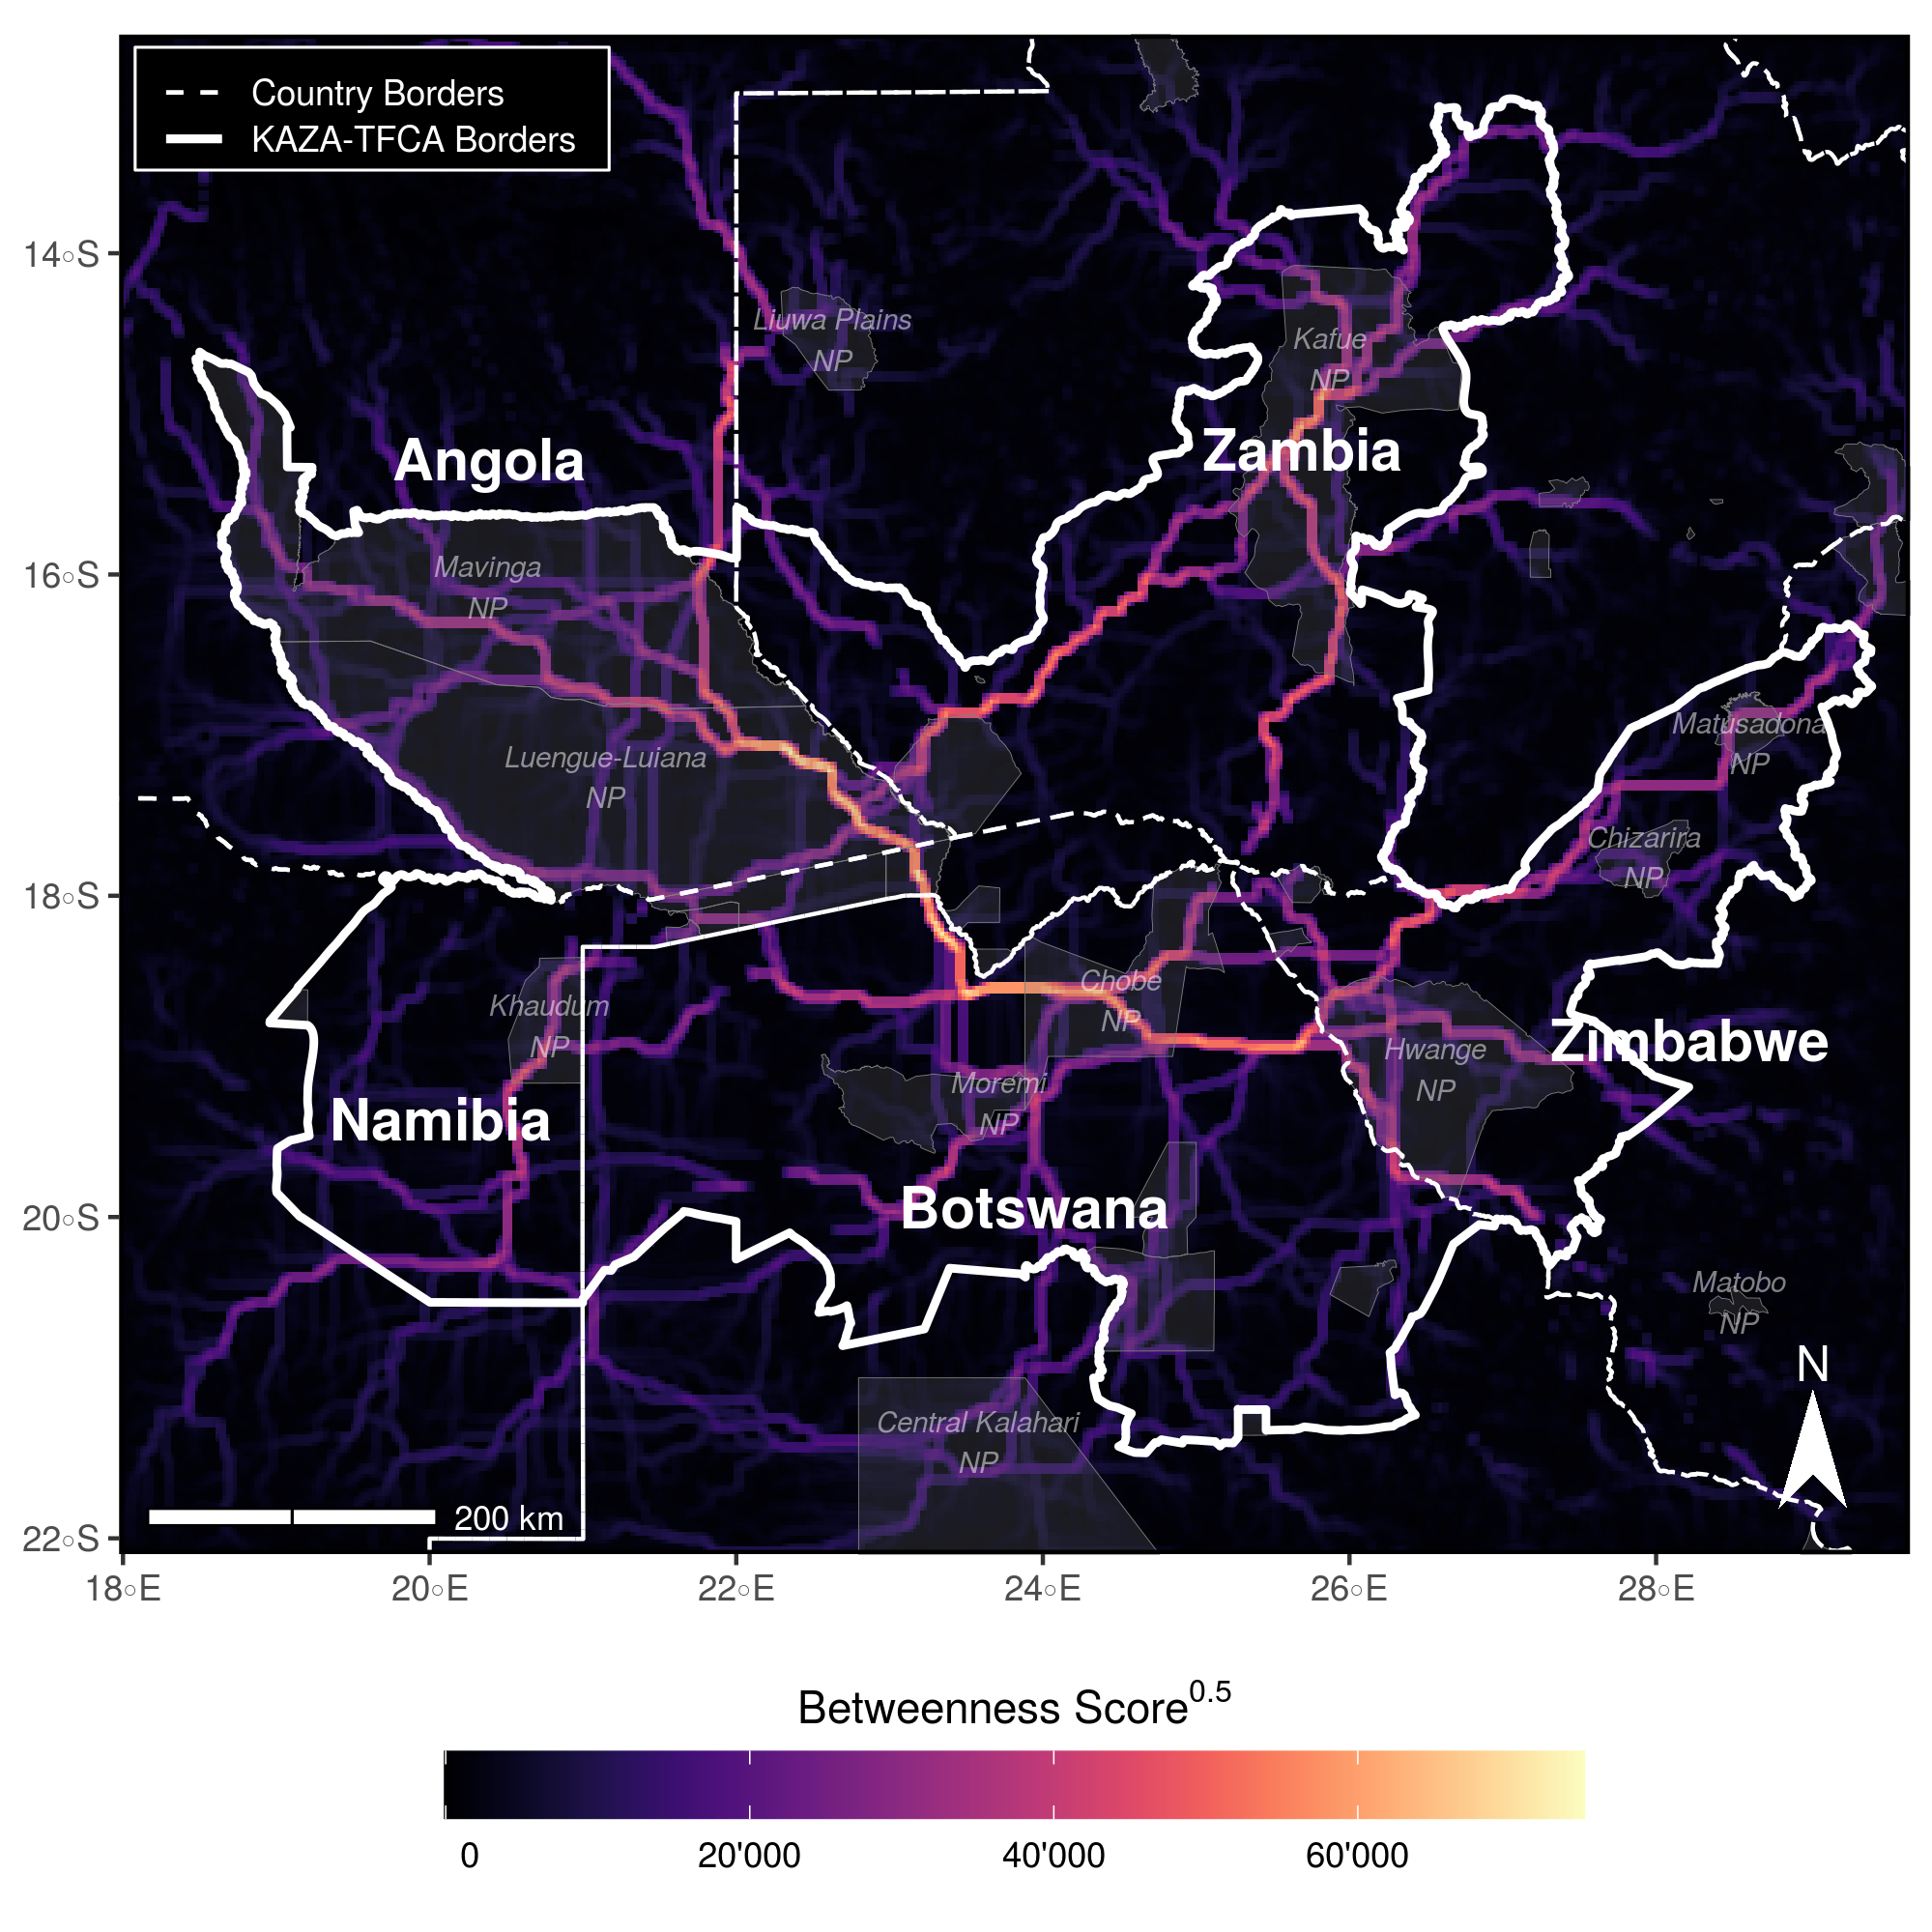
\includegraphics[width=\textwidth]{99_Betweenness.png}
  \caption{Map of betweenness scores, highlighting distinct dispersal corridors
  and potential bottlenecks across the extent of the KAZA-TFCA. Betweenness
  measures the number of shortest paths traversing through each node
  (raster-cell). Hence, a high betweenness score indicates that the respective
  area is exceptionally important for connecting different regions in the study
  area. The metric is therefore useful to pinpoint discrete movement corridors
  \citep{BastilleRousseau.2018}. Note that we square-rooted betweenness scores
  to improve visibility of corridors with comparably low scores. Additional
  betweenness maps showing betweenness scores when individuals move fewer than
  2'000 steps are provided in Figure S4.}
  \label{Betweenness}
\end{figure}

\subsection{Inter-Patch Connectivity}
The inter-patch connectivity map showed that the relative frequency at which
simulated dispersal trajectories moved from one NP to another varied, as did the
average dispersal duration required to make these connections
(\Cref{InterpatchConnectivity}). Overall, inter-patch connectivity between NPs
in Angola, Namibia, Botswana, and Zimbabwe appeared to be high; between 54\% and
87\% of individuals originating from a NP in these countries successfully moved
into some other NP (Figure S7a). Conversely, only 19\% of the dispersers leaving
from a NP in Zambia managed to find a route into some other NP (Figure S7b).
Prior to reaching another NP, individuals from Angola, Namibia, Botswana,
Zimbabwe, and Zambia had to move for an average of 630, 640, 940, 1045, and 890
steps, respectively. For some NPs, we also detected imbalances between the
number of ingoing and outgoing links, hinting at possible source-sink dynamics.
From Chobe NP, for instance, 510 individuals reached Moremi NP, yet the opposite
route was only realized by 340 individuals. However, relative to the number of
simulated individuals, these numbers imply fractions of 50\% and 68\%,
respectively. Furthermore, it appeared that the dispersal corridor between
Angola's NPs and the Kafue NP in Zambia identified in
\Cref{InterpatchConnectivity} is only rarely realized.

\begin{figure}
  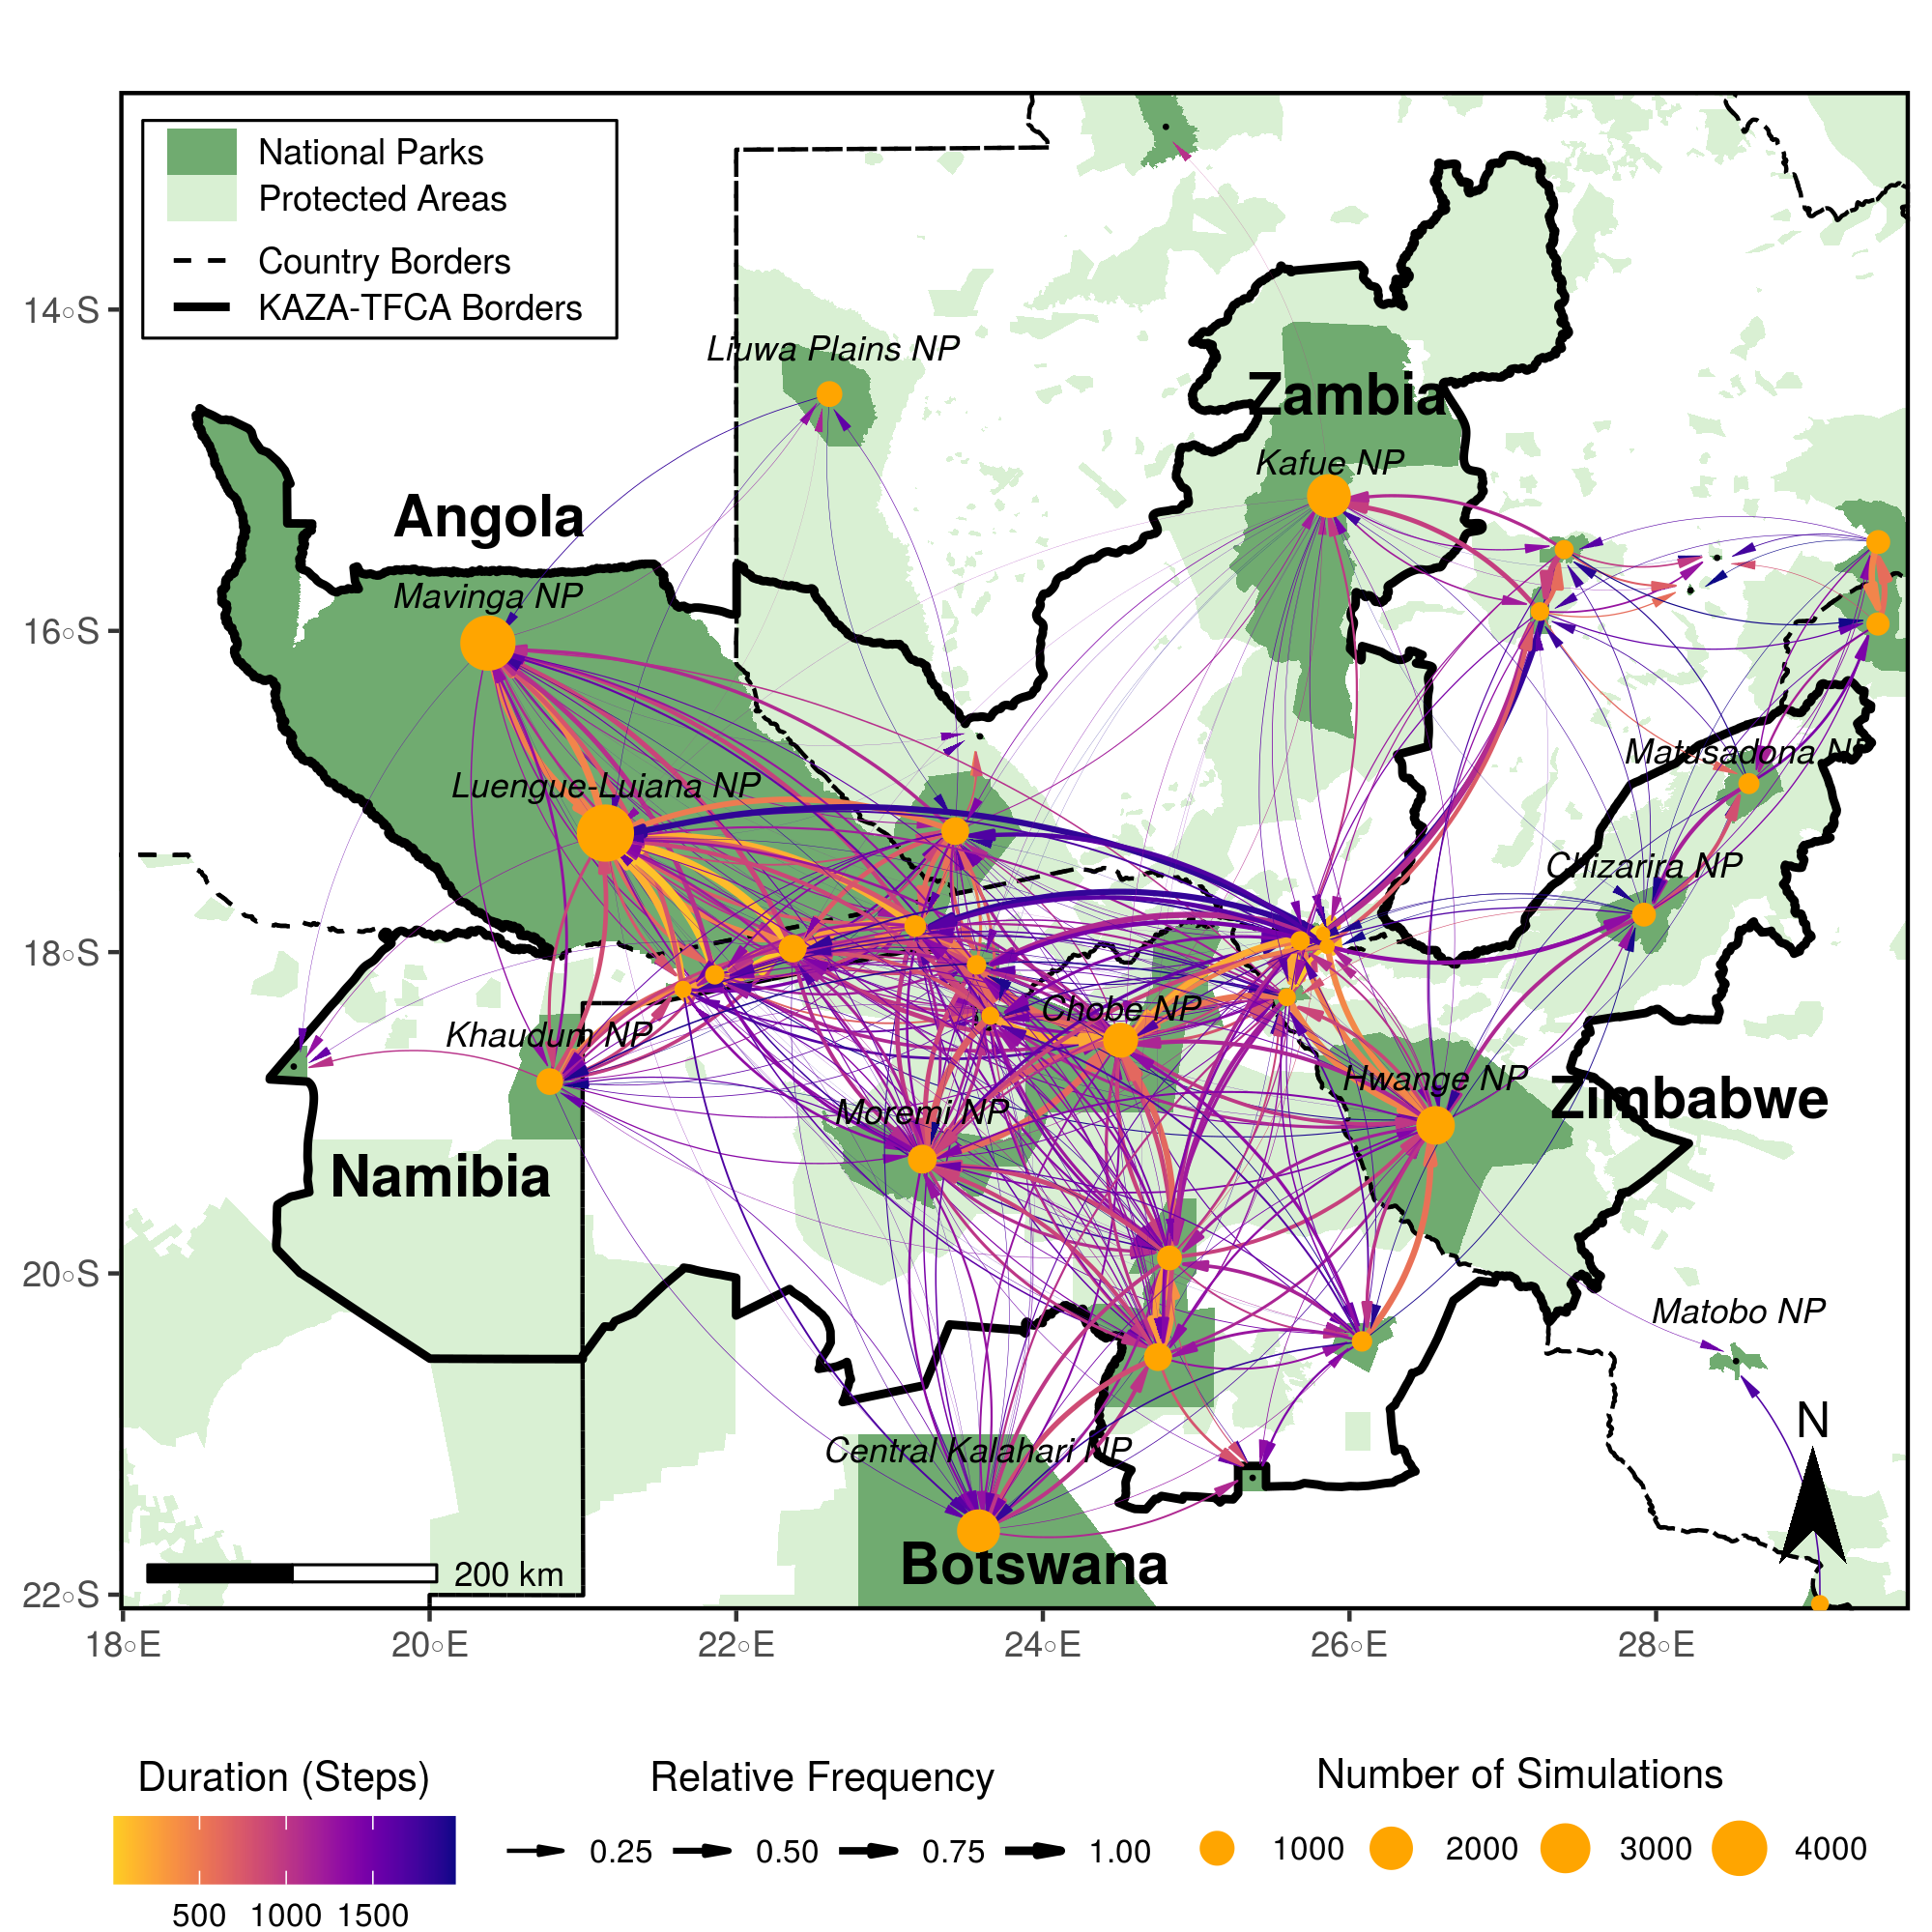
\includegraphics[width=\textwidth]{99_InterpatchConnectivity.png}
  \caption{Map of inter-patch connectivity in relation to dispersal duration,
  highlighting connections between NPs (dark green). Yellow bubbles represent
  the center of the different NPs and are sized in relation to the number of
  simulated dispersers originating from each park. Black dots represent NPs that
  were smaller than 700 km\textsuperscript{2} and therefore did not serve as
  source areas. Arrows between NPs illustrate between which NPs the simulated
  dispersers successfully moved and the color of each arrow shows the average
  number of steps (4-hourly movements) that were necessary to realize those
  connections. Additionally, the line thickness indicates the relative number of
  dispersers originating from a NP that realized those connections. Note that a
  similar network view could be adopted to investigate connectivity between
  other protected areas need not to be restricted to NPs.}
  \label{InterpatchConnectivity}
\end{figure}

\section{Discussion}

% Short Summary
\subsection{Short Summary}
Here, we proposed a three-step approach to assess landscape connectivity via
simulated dispersal trajectories, and demonstrated its application using
empirical data from a free-ranging population of African wild dogs. In step one,
we used ISSFs to parametrize a fully mechanistic movement model describing how
individuals move through the landscape. In step two, we employed the movement
model to simulate dispersal trajectories across the landscape. In step three, we
translated the simulated trajectories into three complementary connectivity
maps, each emphasizing a different aspect of landscape connectivity (e.g.
frequently traversed areas, critical dispersal corridors and bottlenecks, and
the presence and intensity of functional links between suitable patches).
Importantly, such simulations from ISSFs overcome several conceptual
shortcomings inherent to more traditional connectivity modeling techniques, such
as LCPA and CT.

% Movement Model
\subsection{Movement Model}
Our results on habitat preferences showed that dispersers avoid areas dominated
by humans and covered by water, but select for regions with open grassland in
the vicinity to water bodies. This largely complied with previous studies that
investigated habitat selection by dispersing wild dogs
\citep{DaviesMostert.2012, Masenga.2016, Woodroffe.2019, Oneill.2020,
Hofmann.2021}. However, by also accounting for movement preferences, we were
able to model several additional complexities common to dispersal. For instance,
by including an interaction between turning angle and step length we could
accommodate that dispersers exhibit step lengths that are correlated with
turning angles, meaning turning angles are smaller when individuals move fast.
Although similar autocorrelations could be incorporated by sampling step lengths
and turning angles from copula probability distributions \citep{Hodel.2021a,
Hodel.2021b}, the ISSF framework allowed us to conventiently include
correlations in the movement model. We only considered first order
autocorrelation, i.e. correlation between two consecutive steps, although higher
order autocorrelation is conceivable and may be desirable to model
\citep{Dray.2010, McClintock.2012}. This will, however, require vast amounts of
GPS data that are not interrupted by missing fixes; something that is rarely
achieved in reality \citep{Graves.2006}. The power and flexibility of ISSFs to
model additive effects between habitat and movement covariates
\citep{Avgar.2016, Signer.2017} furthermore allowed us to formally capture that
dispersing wild dogs move slower and more tortuous in areas covered by water,
something that surely was to be expected. Overall, the inclusion of interactions
between habitat and movement covariates in our movement model lead to a
significant improvement in predictive performance compared to an earlier model
that omitted such interactions \citep{Hofmann.2021}.

\subsection{Simulation}
While our approach of simulating dispersal proved usedful to assess landscape
connectivity, it was computationally very costly. Our simulation of 80,000
dispersal trajectories moving 2'000 steps across the KAZA-TFCA required five
days of computation on a regular desktop machine (AMD Ryzen 7 2700X processor
with 8 x 3.6 GHz and 16 logical cores, 64 GB of RAM). The long simulation time
was primarily caused by the massive extent of the study area considered (ca. 1.8
Mio km\textsuperscript{2}) and the large number of trajectories simulated. Most
connectivity studies focus on smaller study areas (e.g. \citealp{Kanagaraj.2013,
Clark.2015, McClure.2016, Abrahms.2017, Zeller.2020}) and will therefore achieve
faster simulation times (given the same spatial resolution across covariates).
We also believe that fewer simulated trajectories will often suffice, as the
relative traversal frequency by simulated trajectories through randomly placed
checkpoints across our study area converged already after 10,500 runs. The
number of required simulations to achieve reliable estimates of connectivity
will, however, vary depending on the structure of the landscape and the
dispersal behavior of the focal species \citep{Gustafson.1996}. For species that
disperse short distances through homogeneous environments, few simulations may
suffice to gauge connectivity, whereas for species that disperse over long
distances through heterogeneous habitats, a large number of simulations will be
required to sufficiently explore the spectrum of possible routes.

\subsection{Maps}
Each of the three connectivity maps derived from simulated dispersal
trajectories highlighted a different aspect of landscape connectivity. The
heatmap was most suitable for pinpointing frequently traversed areas and showed
that an exceptionally large number of dispersers moved through the regions of
the Moremi NP and the Chobe NP in northern Botswana. \citep{Hofmann.2021}
previously identified the same area as potential dispersal hotspot using LCPA,
however, it was not clear whether this was the consequence of the central
location of the region and connections being enforced between predefined start
and endpoints. Contrary to LCPA, a simulation-based approach as presented here
does not require predefined endpoints because endpoints, as endpoints emerge
naturally from the simulated dispersal trajectories. Not having to predefine
endpoints is especially useful for dispersal studies, as known endpoints are
usually an unrealistic assumption \citep{Elliot.2014, Abrahms.2017, Cozzi.2020}.
Simulations also enable the detection of potential routes that do not lead into
suitable habitats \citep{Dwernychuk.1972, VanDerMeer.2014} but into areas with a
high susceptibility for human wildlife conflicts \citep{Cushman.2018}.

In contrast to the heatmap, the betweenness map emphasized relatively narrow and
linear movement routes and thus facilitated the identification of discrete
movement corridors. The resulting map reinforced our notion that Botswana plays
a central role for the establishment of connections into more remote regions of
the KAZA-TFCA. While, in this case, both the heatmap and the betweenness map
attributed a high importance to northern Botswana, little consensus was found
for other regions. For instance, the stretch of unprotected land between
Luengue-Luiana NP in Angola and the Kafue NP in Zambia was characterized by a
high betweenness-score, but at the same time received a low heatmap score. These
contrasts highlight the complementary nature of the presented connectivity maps
and emphasize the value of consulting multiple metrics when assessing
connectivity.

Finally, we produced a map of inter-patch connectivity. The map depicted the
frequency at which simulated individuals moved between NPs as well as the
average duration (in steps) required to realize them. Calculating dispersal
durations was possible because dispersal trajectories were simulated spatially
and temporally explicitly, something that is currently impossible with LCPA or
CT. An explicit representation of time enables answerings questions such as:
``\textit{How long will it take a disperser to move from A to B?}'' or
``\textit{Is it possible for a disperser to move from A to B within X days?}''.
Moreover, it yields opportunities to study how seasonality affects connectivity
and to investigate whether dispersal corridors exist seasonally or all-year
round (\textit{dynamic connectivity}; \citealp{Zeller.2020}). With LCPA or CT,
seasonality can currently only be incorporated by repeatedly running a
connectivity analysis using an array of seasonal permeability surfaces (e.g.
\citealp{Benz.2016, Osipova.2019}). In contrast, simulations from ISSFs allow
the environment to change ``as the dispersers move'', so that simulated
trajectories can dynamically respond to seasonal fluctuations in the
environment.

\subsection{Disadvantages of ISSF Simulations}
Despite the many benefits and great flexibility offered by simulations from
ISSFs, one must also be aware of the associated non-trivial but important
modeling decisions. Here, we will further elaborate on four modeling decisions:
(1) the number of simulated individuals, (2) the location of source points, (3)
the simulated dispersal duration, and (4) behavior at map boundaries.

(1) When simulating dispersal trajectories, the modeler needs to decide on the
number of simulated individuals. A higher number is always desirable, as each
additional trajectory provides information about landscape connectivity.
However, each additional simulation entails computational costs, so a trade-off
needs to be managed. Here, we followed \cite{Signer.2017} who suggested to
simulate additional individuals only until the metrics of interest converge
towards a steady state. The exact number of required individuals might, however,
vary depending on the target metric and the anticipated connectivity map.
Consequently, more sophisticated target metrics tailored for each of the
presented connectivity maps need to be developed in the future.

(2) To initiate dispersers, a modeler needs to provide a set of source points at
which the virtual disperser will be released. We placed source points within
protected areas large enough to sustain viable wild dog populations, implicitly
assuming wild dogs primarily survive in large, formally protected areas
\citep{Woodroffe.1999, DaviesMostert.2012, Woodroffe.2012, VanDerMeer.2014}. We
lacked precise knowledge about the presence and abundance of wild dogs in the
different protected areas, so we distributed source randomly points within them.
In cases where such data is available, source points could be distributed
accordingly, reflecting that the number of simulated trajectories does not
necessarily scales with the size of the source area. Alternatively, source
points could be distributed homogeneously and only later be weighted when
computing the heatmap, betweenness map, or inter-patch connectivity map. In any
case, the challenge of selecting meaningful source points is not unique to
individual-based simulations but also applies to LCPA or CT.

(3) The use of ISSFs to simulate dispersers requires deciding on the number of
simulated steps (i.e. dispersal durations). If sufficient dispersal data of the
focal species has been collected, dispersal durations can be sampled from
observed dispersal events. Due to the low number of observed dispersal events,
we opted against this solution and instead simulated all individuals for 2,000
steps, which is at the upper end of observed dispersal durations
\citep{DaviesMostert.2012, Masenga.2016, Cozzi.2020, Hofmann.2021}. This
approach also had the advantage that it allowed us to subsample simulated
trajectories to shorter durations after their simulation and thereby to
investigate the sensitivity of our results with respect to exact dispersal
durations (Figures S4 and S5).

(4) Unless simulated dispersal trajectories are strongly drawn towards a point
of attraction (e.g. \cite{Signer.2017}), some trajectories will inevitably
approach a map boundary and one or more of the generated random steps will leave
the study area. One solution to deal with such cases would be to simply
terminate the simulation of the affected trajectory, implicitly assuming that
the respective animal left the study area. However, this approach might produce
ambiguous results in cases where individuals are released near map borders,
since already a single random step leaving the study area will break the
simulation, thus resulting in biased connectivity estimates along map borders.
Rather than halting the simulation, we created a buffer zone \citep{Koen.2010}
and resampled random steps until they fully lied within the study area. This
proved to be an effective solution to overcome problems with boundary effects.

\subsection{Conclusion}
In summary, we proposed and applied a simple three-step approach that relies on
ISSF-analysis and enables the simulation of dispersal trajectories and the
assessment of landscape connectivity. The proposed approach overcomes several of
the conceptual shortcomings inherent to LCPA and CT, such as the assumption of
known endpoints, and provides a highly flexible tool for investigating
connectivity. With this work, we hope to have sparked interest in the
application, optimization, or creation of methods to investigate dispersal
movements and connectivity via individual-based simulations, while at the same
time stressing some of the non-trivial modeling decisions involved. We also hope
to provide a useful framework that helps unifying and streamlining the
application of individual-based simulation for assessing landscape connectivity.

\section{Authors' Contributions}
D.D.H., D.M.B., A.O. and G.C. conceived the study and designed methodology;
D.M.B., G.C., and J.W.M. collected the data; D.D.H. and D.M.B. analysed the
data; G.C. and A.O. assisted with modeling; D.D.H., D.M.B., and G.C. wrote the
first draft of the manuscript and all authors contributed to the drafts at
several stages and gave final approval for publication.

\section{Data Availability}
GPS movement data of dispersing wild dogs is available on dryad
\citep{Hofmann.2021b}. Access to R-scripts that exemplify the application of the
proposed approach using simulated data are provided through Github
(\url{https://github.com/DavidDHofmann/DispersalSimulation}). In addition, all
codes required for the African wild dog case study will be made available
through an online repository at the time of publication.

\section{Acknowledgements}
We thank the Ministry of Environment and Tourism of Botswana for granting
permission to conduct this research. We thank C. Botes, I. Clavadetscher, and G.
Camenisch for assisting with wild dog immobilizations. We also thank B. Abrahms
for sharing her data of three dispersing wild dogs. Furthermore, we would like
to thank Johannes Signer for assisting with the simulation algorithm. This study
was funded by Albert-Heim Foundation, Basler Stiftung für Biologische Forschung,
Claraz Foundation, Idea Wild, Jacot Foundation, National Geographic Society,
Parrotia Stiftung, Stiftung Temperatio, Wilderness Wildlife Trust Foundation,
Forschungkredit der Universität Zürich, and a Swiss National Science Foundation
Grant (31003A\_182286) to A. Ozgul.

\newpage
\begingroup
\singlespacing
\bibliography{Literatur}
\endgroup

\end{document}
